\section{Performance Evaluation}

To evaluate the efficacy of each classifier, we made a function to extract the values from the confusion matrix of the ensemble of 20 forests. This function then calculates the True Positive and False Positive Rates to be plotted in a ROC curve. Here, the threshold we vary is the percent of Random Forests in the whole ensemble required to predict ``True'' before the ensemble as a whole will predict ``True'' (where True means we predict the contest will not fill). By plotting multiple ROC curves on the same graph, we found it relatively easy to divine which methodology of classification was most effective. A better performing predictor will always tend towards the top left corner (i.e. have a larger area under it's curve).

\begin{table}
\begin{center}
\begin{tabular}{| c | c | c | c | c | c | c |}
\hline
 \textbf{Contest} & \textbf{Forest 1} & \textbf{Forest 2} & \textbf{Forest 3} & \textbf{Forest 4} & \textbf{Forest 5} & \textbf{True Value} \\ 
 \hline
 Contest 1 & 1 & 1 & 1 & 1 & 1 & 1 \\  
 \hline
 Contest 2 & 0 & 1 & 0 & 0 & 1 & 0 \\
 \hline
 Contest 3 & 0 & 0 & 0 & 1 & 0 & 1 \\
 \hline
 Contest 4 & 1 & 1 & 1 & 0 & 0 & 1 \\
 \hline
 Contest 5 & 0 & 1 & 0 & 1 & 1 & 0 \\
 \hline
 Contest 6 & 0 & 1 & 1 & 0 & 1 & 0 \\
 \hline
 Contest 7 & 1 & 0 & 1 & 1 & 1 & 0 \\
 \hline
 Contest 8 & 1 & 1 & 0 & 0 & 0 & 1 \\
 \hline
 Contest 9 & 1 & 1 & 0 & 1 & 1 & 0 \\
 \hline
 Contest 10 & 1 & 0 & 0 & 0 & 1 & 1 \\
 \hline
\end{tabular}
\caption[Example of Random Forest Predictions]{An example set of predictions from 5 different Random Forests on 10 different contests.}
\end{center}
\end{table}

\begin{table}
\begin{center}
\begin{tabular}{| c | c | c |}
\hline
 \textbf{Contest} & \textbf{Overall Prediction} & \textbf{True Value}\\ 
 \hline
 Contest 1 & 1 & 1 \\  
 \hline
 Contest 2 & 0 & 0 \\
 \hline
 Contest 3 & 0 & 1 \\
 \hline
 Contest 4 & 1 & 1 \\
 \hline
 Contest 5 & 0 & 0 \\
 \hline
 Contest 6 & 1 & 0 \\
 \hline
 Contest 7 & 1 & 0 \\
 \hline
 Contest 8 & 0 & 1 \\
 \hline
 Contest 9 & 1 & 0 \\
 \hline
 Contest 10 & 1 & 1 \\
 \hline
\end{tabular}
\caption[Example of Final Predictions Against True Outcomes]{One possible set of overall predictions from the example data in Table 3.7 for when the threshold for predicting a value of 1 is 60\% (i.e. 3 of the forests must predict 1 in order to have an overall prediction of 1).}
\end{center}
\end{table}

Consider the example data set in Table 3.7. If we use a threshold of 50\%, the overall prediction matrix appears in Table 3.8. Comparing these values to the known True Values, we can produce the confusion matrix in Table 3.9. From this, we can see that with a threshold of 60\% we get an overall accuracy of 30\% with a True Positive Rate of 0.4 and a False Positive Rate of 0.8. Expanding this to all possible thresholds we get the blue ROC curve found in Figure 3.1.

Since this curve appears to be concave up (as opposed to concave down) the area under the curve is fairly small. In fact, because it falls below the line of True Positive Rate = False Negative Rate, we can conclude that the classifier does a very poor job of discerning between 1 and 0 response types and would be better off randomly guessing. However, we could also invert this line by inverting every predicted value. Doing so would produce the orange curve seen in Figure 3.1 which appears to do reasonably well at classification based on the increased area under its curve.

\begin{table}
\centering
\begin{tabular}{| c | c | c |}
\hline
 & \textbf{Predict 0} & \textbf{Predict 1}  \\ 
\hline
\textbf{Actually 0} & 2 & 3 \\ 
\hline
\textbf{Actually 1} & 2 & 3 \\
\hline
\end{tabular}
\caption[Our Example's Confusion Matrix]{The confusion matrix for the set of predictions shown in Table 3.8 when compared against their respective known True Values.}
\end{table}

\begin{figure}[h]
\centering
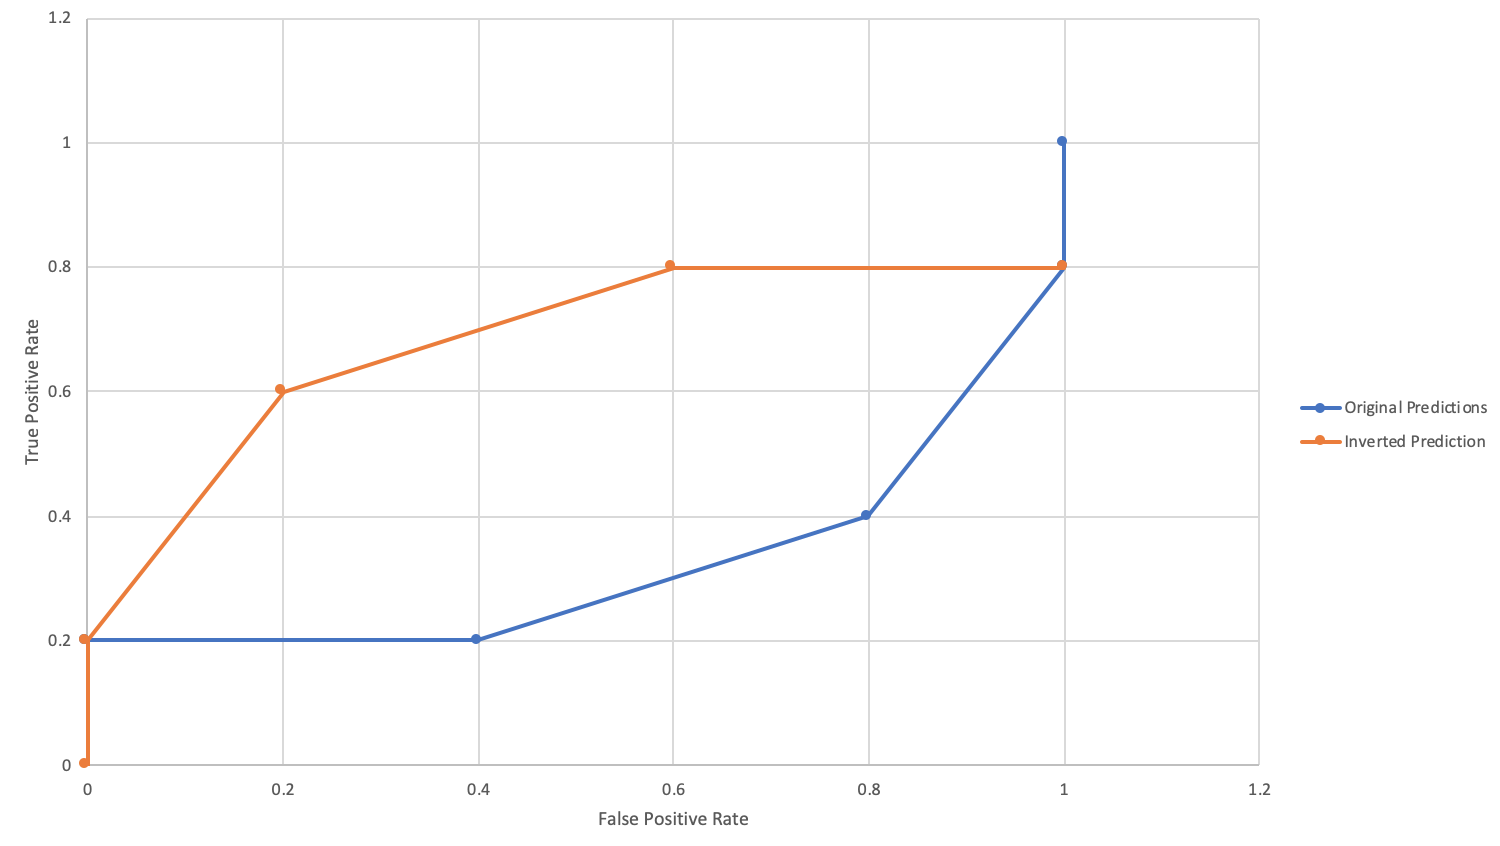
\includegraphics[width=10cm]{body/methodology/Both_ROC.png}
\caption[Combined ROC Curve for a Sample Classification]{In Blue: the ROC curve generated by varying the prediction threshold for the ensemble of forests. In Orange: the ROC curve generated by taking the opposite of every prediction for each threshold of the ensemble of forests.}
\end{figure}

